% This file was created by matlab2tikz.
%
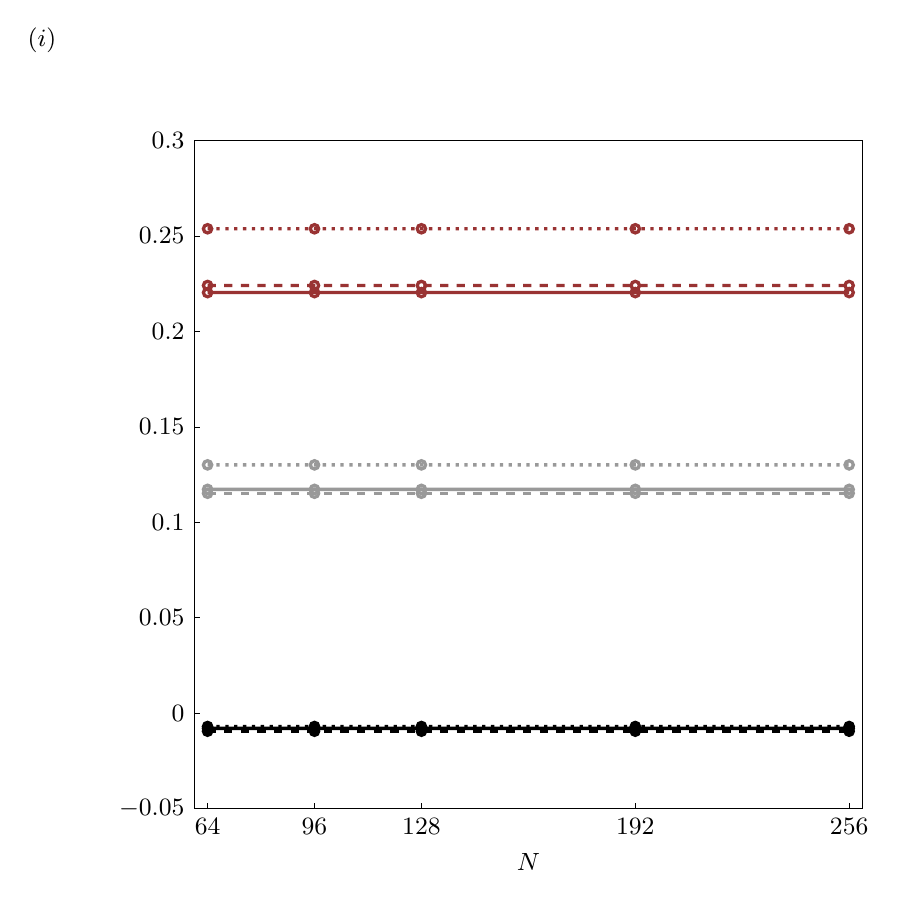
\begin{tikzpicture}

\begin{axis}[%
width=11.255in,
height=7.131in,
at={(1.888in,0.962in)},
scale only axis,
clip=true,
separate axis lines,
every outer x axis line/.append style={black},
every x tick label/.append style={font=\color{black}},
every x tick/.append style={black},
xmin=60,
xmax=260,
xtick={ 64,  96, 128, 192, 256},
xlabel={$N$},
every outer y axis line/.append style={black},
every y tick label/.append style={font=\color{black}},
every y tick/.append style={black},
ymin=-0.05,
ymax=0.3,
axis background/.style={fill=white},
clip=true,
clip mode=individual,
axis lines=box,
xtick pos=bottom,
ytick pos=left,
tick align=inside,
major tick length=2pt,
width=0.7\linewidth,
height=0.7\linewidth,
every axis/.append style={font=\fontsize{9}{9}\selectfont},xlabel style={font=\fontsize{9}{9}\selectfont},title style={font=\fontsize{9}{9}\selectfont},
legend style={font=\fontsize{8}{9}\selectfont,inner sep=1pt,row sep=1pt,column sep=2pt,nodes={scale=1.00},draw=none},legend image post style={xscale=0.35},
legend columns=1,
scaled x ticks=false,
tick label style={/pgf/number format/fixed,/pgf/number format/precision=2},
every x tick label/.append style={font=\fontsize{9}{9}\selectfont\color{black}},
every y tick label/.append style={font=\fontsize{9}{9}\selectfont\color{black}},
,,
colormap={sigmamap}{rgb(0.0000)=(0.0200,0.1880,0.3800); rgb(0.1000)=(0.0743,0.3456,0.5616); rgb(0.2000)=(0.1918,0.4980,0.7060); rgb(0.3000)=(0.3890,0.6708,0.8226); rgb(0.4000)=(0.7552,0.8682,0.9228); rgb(0.5000)=(0.9690,0.9689,0.9689); rgb(0.6000)=(0.9425,0.8044,0.7614); rgb(0.7000)=(0.8767,0.4910,0.4020); rgb(0.8000)=(0.7869,0.2866,0.2470); rgb(0.9000)=(0.6186,0.1239,0.1568); rgb(1.0000)=(0.4040,0.0000,0.1220)}
]
\addplot [color=black, line width=1.2pt, mark size=1.5pt, mark=o, mark options={solid, black}, forget plot]
  table[row sep=crcr]{%
64	-0.00792566236976146\\
96	-0.00792568606431545\\
128	-0.00792568601830253\\
192	-0.00792568601891497\\
256	-0.00792568601868533\\
};
\addplot [color=black, dashed, line width=1.2pt, mark size=1.5pt, mark=o, mark options={solid, black}, forget plot]
  table[row sep=crcr]{%
64	-0.00941347284988948\\
96	-0.00941347291006718\\
128	-0.00941347290991271\\
192	-0.00941347290970737\\
256	-0.00941347291074579\\
};
\addplot [color=black, dotted, line width=1.2pt, mark size=1.5pt, mark=o, mark options={solid, black}, forget plot]
  table[row sep=crcr]{%
64	-0.0069763966934395\\
96	-0.00697642867852829\\
128	-0.0069764286295014\\
192	-0.00697642862853563\\
256	-0.00697642863090525\\
};
\addplot [color=white!60!black, line width=1.2pt, mark size=1.5pt, mark=o, mark options={solid, white!60!black}, forget plot]
  table[row sep=crcr]{%
64	0.117214354250601\\
96	0.11721437286601\\
128	0.117214372698788\\
192	0.117214372690895\\
256	0.117214372696531\\
};
\addplot [color=white!60!black, dashed, line width=1.2pt, mark size=1.5pt, mark=o, mark options={solid, white!60!black}, forget plot]
  table[row sep=crcr]{%
64	0.115201027728144\\
96	0.115201032663785\\
128	0.115201032665002\\
192	0.115201032658196\\
256	0.115201032656291\\
};
\addplot [color=white!60!black, dotted, line width=1.2pt, mark size=1.5pt, mark=o, mark options={solid, white!60!black}, forget plot]
  table[row sep=crcr]{%
64	0.130051378102756\\
96	0.130051336342246\\
128	0.130051336263221\\
192	0.130051336259834\\
256	0.130051336265891\\
};
\addplot [color=red!60!teal, line width=1.2pt, mark size=1.5pt, mark=o, mark options={solid, red!60!teal}, forget plot]
  table[row sep=crcr]{%
64	0.220279754122664\\
96	0.220280257995508\\
128	0.220280259137585\\
192	0.220280259149969\\
256	0.220280259136001\\
};
\addplot [color=red!60!teal, dashed, line width=1.2pt, mark size=1.5pt, mark=o, mark options={solid, red!60!teal}, forget plot]
  table[row sep=crcr]{%
64	0.224001540833978\\
96	0.224001035040474\\
128	0.224001034229596\\
192	0.224001034240017\\
256	0.224001034230161\\
};
\addplot [color=red!60!teal, dotted, line width=1.2pt, mark size=1.5pt, mark=o, mark options={solid, red!60!teal}, forget plot]
  table[row sep=crcr]{%
64	0.253693751107552\\
96	0.253697223035508\\
128	0.253697220159432\\
192	0.253697220121145\\
256	0.253697220175179\\
};
\node[right, align=left, inner sep=0]
at (rel axis cs:-0.25,1.15) {$(i)$};
\end{axis}
\end{tikzpicture}%